\documentclass{assignment}

\usepackage{float}
\usepackage{tikz}
\usepackage{adjustbox}
\usepackage{titlesec}
\usepackage{soul}
\usepackage{csvsimple}

\usepackage{bm}
\usepackage{amsmath,amssymb}

\usepackage{pgfplots}
\usepackage{graphics, epsfig}

\usepackage{graphicx}
\usepackage{subcaption}
\usepackage{matlab-prettifier}
\usepackage{multirow}

\usetikzlibrary{decorations.pathmorphing, decorations.markings}
\usetikzlibrary{positioning}

\usetikzlibrary{calc,patterns,angles,quotes}
\setlength{\parindent}{0pt}

\usetikzlibrary{shapes, arrows}
\tikzstyle{startstop} = [rectangle, rounded corners, minimum width=3cm, minimum height=1cm, text centered, draw=black, fill=red!30]
\tikzstyle{io} = [trapezium, trapezium stretches=true, trapezium left angle=70, trapezium right angle=110, minimum width=4cm, minimum height=1cm, text centered, draw=black, fill=blue!30]
\tikzstyle{process} = [rectangle, minimum width=4cm, minimum height=1cm, text centered, text width=4cm, draw=black, fill=orange!30]
\tikzstyle{decision} = [diamond, minimum width=3cm, minimum height=1cm, text centered, draw=black, fill=green!30]
\tikzstyle{arrow} = [thick,->,>=stealth]

\hypersetup{
pdftitle={Autonomous Vehicles},
pdfsubject={Project for the course of Autonomous Vehicles},
pdfauthor={Tommaso Bocchietti}
}

\makeglossaries

\begin{document}

\title{Autonomous Vehicles \\ Implementation of sampled-based motion planning algorithms}
\author{Tommaso Bocchietti 10740309}
\date{A.Y. 2024/25}

\maketitle

\begin{figure}[H]
    \centering
    \includegraphics[width=0.7\textwidth]{./pdf/Polimi_logo_coverpage.pdf}
    \label{fig:Polimi_logo}
\end{figure}

\clearpage
\tableofcontents
\listoffigures
% \listoftables
% \lstlistoflistings
% \printglossary[type=\acronymtype]

\clearpage
\section{Introduction}
\label{sec:introduction}

The aim of this work is to gain insight into the development of a feedback control loop for an autonomous vehicle, specifically a \texttt{Turtlebot3} robot of the model \texttt{burger}.
Two different control strategies have been implemented, namely a simple proportional controller and a non-linear controller based on Lyapunov stability theory.
As for the simulation environment, the \texttt{Turtlebot3} robot was simulated in a Gazebo world, specifically the \texttt{turtlebot3\_world} provided by the \texttt{turtlebot3\_gazebo} package.

The following sections provide a detailed description of the requests associated with this assignment, the approach taken to fulfill them, and the discussion of the results obtained.

\paragraph{Tools}

As for the tools used, \texttt{ROS1} (Robot Operating System) is employed as the main framework for communication between the different components of the system.
\texttt{Simulink} is used as the main agent in the loop, sending control commands to the vehicles based on the telemetry data received from the vehicle itself.
\texttt{MATLAB} instead is used to perform the analysis of the data collected during the simulation, and to visualize the results.
Notice that with the current setup used by the author, \texttt{MATLAB 2024a} and \texttt{Simulink} are running in Windows 10, while \texttt{ROS1} is running in the \texttt{WSL2} (Windows Subsystem for Linux) environment, specifically in the \texttt{Ubuntu 22.04} distribution.

\section{Sampling-based planning}
\label{sec:sampling_based_planning}

In the field of robotics, a variety of algorithms are available for path planning, each with its own strengths and weaknesses.
One of the most ancient and well known class of algorithms is the so called \textit{Grid-based}, which is based on the discretization of the environment into a grid of cells and nodes.
As we have already discovered during the previous assignment, this approach is particularly useful for environments with a known structure, such as indoor environments or outdoor environments with well-defined obstacles but is limited in terms of scalability and flexibility.

In contrast, \textit{Sampling-based} algorithms are designed to work in high-dimensional spaces and can handle much more complex environments.
For this reason, most of the modern path planning algorithms are based on sampling-based methods, which are able to efficiently explore the configuration space of the robot and find a feasible path from the start to the goal configuration.

Among the many robotics applications that benefit from sampling-based algorithms, we can mention:

\begin{itemize}
    \item Terrestrial robots: path planning for autonomous vehicles in outdoor environments, such as urban areas or off-road terrains. The ability to handle large environments is crucial for the success of these applications.
    \item Robotic manipulation: path planning for robotic arms in cluttered environments, where the robot needs to avoid obstacles and reach a specific target position. The ability to handle high-dimensional configuration spaces is essential for these applications.
\end{itemize}

Sampling-based algorithms are further divided into two main classes: \textit{single-query} and \textit{multi-query} algorithms.
Single-query algorithms are designed to find a path from a specific start configuration to a specific goal configuration, while multi-query algorithms are designed to find paths between multiple pairs of start and goal configurations.

In the following sections, we focus exclusively on the single-query algorithms, leaving the multi-query algorithms for future discussions.


\subsection{Single-query algorithms}
\label{sec:single_query_algorithms}

As it was for the grid-based ones, also the single-query sampling-based algorithms follow a structure that is in common to all of them.
The main idea here is to start from a given configuration and then randomly sample points in the configuration space, connecting them to form a tree if the condition of collision-free is satisfied.
The tree is then incrementally expanded until a path from the start configuration to the goal configuration is found.

The fundamental difference between grid-based and sampling-based algorithms is that the former rely on a discretized representation of the environment, while the latter rely on a continuous representation of the configuration space.
This allows sampling-based algorithms to handle complex environments with arbitrary shapes and obstacles, as they do not rely on a fixed grid structure.

\begin{figure}[H]
    \centering

    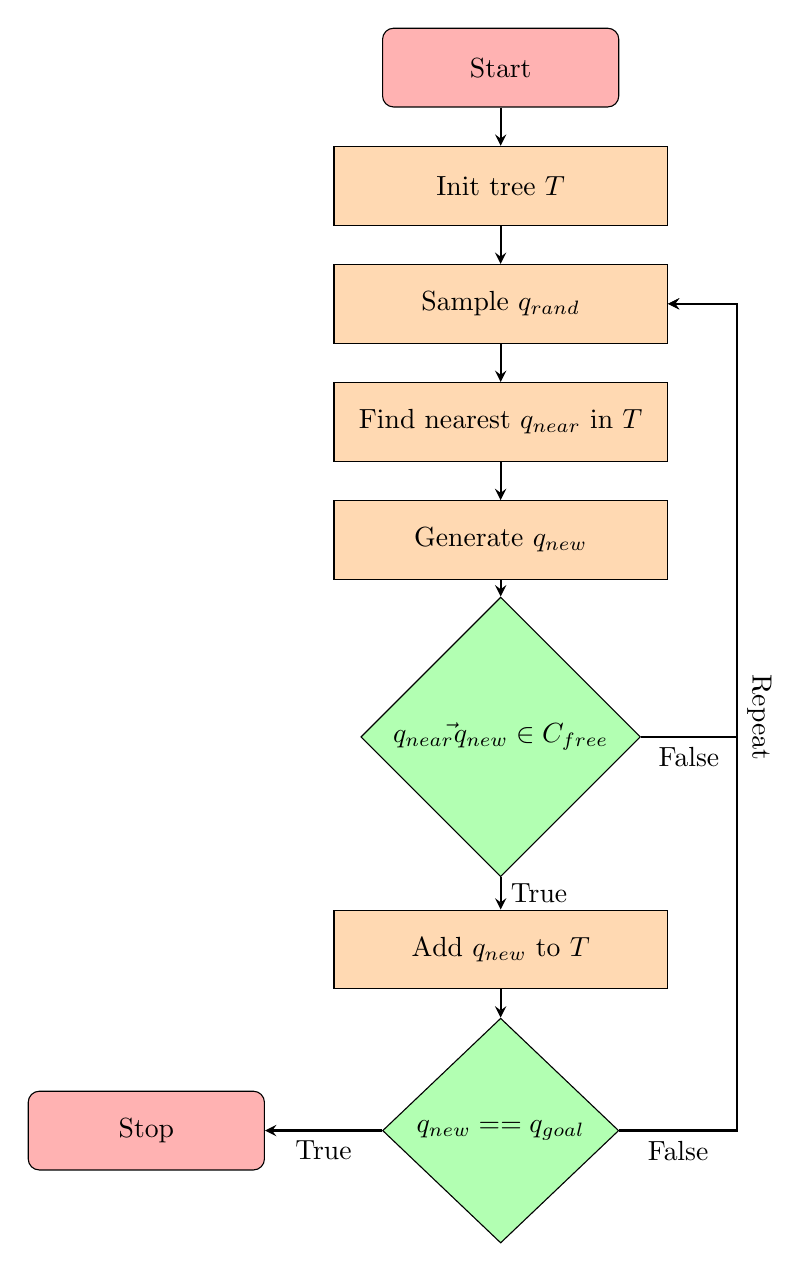
\begin{tikzpicture}[node distance=1.5cm]

        % Nodes
        \node (start) [startstop] {Start};
        \node (init) [process, below of=start] {Init tree $T$};
        \node (sample) [process, below of=init] {Sample $q_{rand}$};
        \node (nearest) [process, below of=sample] {Find nearest $q_{near}$ in $T$};
        \node (new) [process, below of=nearest] {Generate $q_{new}$};
        \node (collision) [decision, below of=new, yshift=-1.0cm] {$\vec{q_{near}q_{new}} \in C_{free}$};
        \node (add) [process, below of=collision, yshift=-1.2cm] {Add $q_{new}$ to $T$};
        \node (end) [decision, below of=add, yshift=-0.8cm] {$q_{new} == q_{goal}$};

        \node (stop) [startstop, left of=end, xshift=-3cm] {Stop};

        % Arrows
        \draw [arrow] (start) -- (init);
        \draw [arrow] (init) -- (sample);
        \draw [arrow] (sample) -- (nearest);
        \draw [arrow] (nearest) -- (new);
        \draw [arrow] (new) -- (collision);
        \draw [arrow] (collision) -- node[anchor=west] {True} (add);
        \draw [arrow] (collision) -- node[anchor=north] {False} +(3,0) |- (sample.east);
        \draw [arrow] (add) -- (end);
        \draw [arrow] (end) -- node[anchor=north] {False} +(3,0) |- (sample.east) node[pos=0.25, above, rotate=-90] {Repeat};
        \draw [arrow] (end.west) -- node[anchor=north] {True} (stop);

    \end{tikzpicture}

    \caption{Generic sampling-based algorithm flowchart}
    \label{fig:sampling_based_flowchart}

\end{figure}

The flowchart in Figure \ref{fig:sampling_based_flowchart} summarizes the main steps of a generic sampling-based algorithm.
One can notice that tree $T$ is built incrementally at each iteration, starting from the initial configuration and adding new sampled points to the tree if they respect the collision-free condition.
As already said, this is in fact the main difference between the sampling-based algorithms and the grid-based algorithms, which rely on a complete discretization of the environment made in advance.

However, the sampling-based algorithms suffers from a major drawback, which is the lack of completeness and optimality.
In particular, the algorithms are not guaranteed to find a solution, even if one exists, and the solution found may not be optimal.
As we discuss in the following sections, improvements have been made to the core structure to address these issues, but they still remain a challenge in the field of robotics and motion planning.

There exist many variations built on top of the core algorithm presented in Figure \ref{fig:sampling_based_flowchart}.
The most common ones are:

\begin{itemize}
    \item \textbf{Rapidly-exploring Random Tree (RRT)}: a single-query algorithm that just implements the core algorithm presented in Figure \ref{fig:sampling_based_flowchart}. It's the simplest, but also the most suboptimal algorithm among the ones presented in this project.
    \item \textbf{RRT*}: an extension of the RRT algorithm that improves the optimality of the solution by rewiring the tree to find shorter paths. It is more computationally expensive than the RRT algorithm, but it is able to refine the solutions in terms of path length.
    \item \textbf{RRT-connect}: a variant of the RRT algorithm that builds two trees, one from the start configuration and one from the goal configuration, and connects them to find a path. It's usually faster than the RRT algorithm to find a solution given that the search space is explored from both ends and also benefits from some form of optimality.
    \item \textbf{RRT-kinematic}: a variant of the RRT algorithm that takes into account the kinematic constraints of the robot/vehicle during the planning process. This is particularly useful for vehicles with non-holonomic constraints, such as terrestrial vehicles or mobile robots. The algorithm generates a tree of feasible trajectories that respect the kinematic constraints of the robot.
\end{itemize}

The following sections focus on the in-depth analysis and implementation of the RRT, RRT* and RRT-kinematic algorithms.
Notice that despite being a popular and widely used algorithm, the RRT-connect algorithm is not going to be implemented in this project due to time constraints.

\section{Algorithm implementation}
\label{sec:algorithm_implementation}

In this section, we present the implementation of the three algorithms we are going to analyze in this report.
The algorithms are implemented in \texttt{MATLAB} and are designed to handle multiple dimensions problems, meaning that they can be used for both N-D environments.
In the following only the core of each algorithm is presented, leaving the code of all the auxiliaries classes such as \texttt{Graph}, \texttt{Edge}, or \texttt{Node} among the files in the repository.


\subsection{RRT algorithm}
\label{subsec:rrt_algorithm}

The most basic version of the single-query sampling-based algorithm is the Rapidly-exploring Random Tree (RRT) algorithm.
The RRT algorithm is nothing more than the direct implementation of the core algorithm presented in Figure \ref{fig:sampling_based_flowchart}.

Listing \ref{lst:rrt_algorithm} shows a possible implementation of the RRT algorithm.

\lstinputlisting[
    style=Matlab-editor,
    caption={Node class used to represent a node in the graph.},
    label={lst:rrt_algorithm}
]{files/rrt.m}


The algorithm takes as input the graph $G$, the map $M$, the start node $s$, and the goal node $g$.
It starts by initializing the tree $T$ with the start node and enters a loop where at first a random point/configuration is sampled from the workspace.
Then, it finds the nearest node already in the tree and generates a new node by moving in the direction of the sampled point.
If the new node is in collision with the obstacles, it's discarded and the algorithm skips to the next iteration.
If the new node is valid, it's added to the tree.
A final step is to check if the new node is close enough to the goal node, in which case the algorithm terminates and returns the path from the start node to the goal node, otherwise the algorithm continues to sample new points until a maximum number of iterations is reached, or the goal node is reached.

The RRT algorithm is simple and efficient, but lacks optimality in the generated path which is normally jagged and not smooth.
The algorithm is also not complete, meaning that it may not find a solution even if one exists in the configuration space due to the maximum number of iterations limit.
However, it has been proved that the RRT algorithm is probabilistically complete, meaning that as the number of iterations increases, the probability of finding a solution approaches 1 (at the cost of longer computation time, of course).



\subsection{RRT* algorithm}
\label{subsec:rrt_star_algorithm}

RRT* is an extension of the RRT algorithm that improves the optimality of the solution by rewiring the tree to find shorter paths.
The main idea behind the RRT* algorithm is to keep track of the cost of reaching each node in the tree and to rewire the tree whenever a new node is added.
This is done by checking if the new node can be used as a cheaper parent connection for any of the existing nodes in the tree.

Listing \ref{lst:rrt_star_algorithm} shows a possible implementation of the RRT* algorithm.

\lstinputlisting[
    style=Matlab-editor,
    caption={Code for the implementation of RRT* algorithm.},
    label={lst:rrt_star_algorithm}
]{files/rrtStar.m}


Again, the core structure of the algorithm is similar to the RRT algorithm, but with a few extra steps.
The algorithm starts by initializing the tree $T$ with the start node and enters a loop where it samples a random point in the configuration space.
Then, it finds the nearest node in the tree and generates a new node by moving towards the sampled point.
If the new node is in collision with the obstacles, it is discarded and the algorithm continues to sample a new point.
If the new node is valid, the algorithm at first connect it to the nearest node in the tree, and then checks if any of its neighbors can also be connected to it with a lower cost-to-go.
This analysis, called rewiring, help to construct a more optimal tree with smoother connections and consequently shorter paths.
Figure \ref{fig:rrt_star} shows an example of the rewiring process.

\begin{figure}[H]
    \centering
    \includegraphics[width=1.0\textwidth]{./img/rrt_star.png}
    \caption{Example of the rewiring process in RRT* algorithm. Credit to \cite{JIANG20244303}.}
    \label{fig:rrt_star}
\end{figure}

As it is going to be shown in the next section, the RRT* algorithm is more efficient than the RRT algorithm in terms of path length, at the cost negligible increase in computation time.

\paragraph{Optimality convergence of RRT*}

As a final note, we recall that thanks to \cite{rrt_optimality}, it has been proved that the RRT* algorithm converges to the optimal solution as the number of sampled points goes to infinity and the rewiring radius is dynamically adjusted as:

\begin{equation}
    r_n = \gamma \left( \frac{\log{n}}{n} \right) ^ {\frac{1}{d+1}}
\end{equation}

Where $n$ is the number of sampled points, $d$ is the dimension of the configuration space, and $\gamma$ is a constant that depends on $d$.

Line 50 of the code in Listing \ref{lst:rrt_star_algorithm} shows a possible implementation of this dynamic rewiring radius.



\subsection{RRT-kinematic algorithm}
\label{subsec:rrt_kinematic_algorithm}

Finally, we move to the last algorithm we are going to implement, which is the RRT-kinematic algorithm.
The RRT-kinematic algorithm is a variant of the RRT algorithm that takes into account the kinematic constraints of the robot during the planning process.
This is particularly useful for vehicles with non-holonomic constraints, such as terrestrial vehicles or mobile robots.

Listing \ref{lst:rrt_kinematic_algorithm} shows a possible implementation of the RRT-kinematic algorithm.

\lstinputlisting[
    style=Matlab-editor,
    caption={Code for the implementation of RRT-kinematic algorithm.},
    label={lst:rrt_kinematic_algorithm}
]{files/rrtKinematic.m}

Again, we recognize the same core structure of the RRT algorithm, but with a few extra steps.
In particular, the choice of the new node is not done by simply moving towards the sampled point, but rather by generating a trajectory from the nearest node in the tree to the sampled point leveraging the kinematic model of the robot.
In the specific case of the implemented algorithm, we consider dealing with a \textit{Bicycle} model, which is a common model used to represent the motion of a car-like vehicle.
Starting from the nearest node in the tree, a random control input is sampled and a trajectory is generated by integrating the kinematic model of the robot over a fixed time horizon.
Collision checking is then performed and among all the tested trajectories, the one that is valid and has the lowest cost is selected as the new node to be added to the tree.
By doing so, we are sure that the generated path is feasible by the robot, respecting its kinematic constraints.

\paragraph{Bicycle kinematic model}

Even if the kinematic model of the vehicle is not the main focus of this report, we briefly present it here for completeness.
The kinematic model of the vehicle is described by the following equations:

\begin{figure}[H]

    \begin{minipage}{0.30\textwidth}

        \begin{equation}
            \begin{aligned}
                \dot{x}      & = v \cdot \cos(\theta)           \\
                \dot{y}      & = v \cdot \sin(\theta)           \\
                \dot{\theta} & = \frac{v}{L} \cdot \tan(\delta)
            \end{aligned}
        \end{equation}

    \end{minipage}
    %
    \hfill
    %
    \begin{minipage}{0.50\textwidth}

        \centering
        \includegraphics[width=1.0\textwidth]{./img/bicycle_model.png}

    \end{minipage}

    \caption{Bicycle kinematic model. Image credit to \href{https://thomasfermi.github.io/Algorithms-for-Automated-Driving/Control/BicycleModel.html}{Thomas Fermi}.}
    \label{fig:bicycle_model}

\end{figure}

Where $x$ and $y$ are the position of the vehicle in the workspace, $\theta$ is the heading angle of the vehicle, $v$ is the linear velocity, $L$ is the wheelbase of the vehicle (distance between the front and rear axles), and $\delta$ is the steering angle.

One can clearly see that the kinematic model is composed by a set of differential equations.
In order to simulate in time based on the control inputs and current state of the vehicle, we need to integrate these equations.
Different integration methods can be used, such as Euler integration or Runge-Kutta integration.
However, given the simplicity and expected slow dynamics of the model, we can use a simple Euler integration with a fixed time step $\Delta t$.

Listing \ref{lst:vehicle_model} shows a possible implementation of the kinematic model of the vehicle.

\lstinputlisting[
    style=Matlab-editor,
    caption={Code for the kinematic model of the vehicle.},
    label={lst:vehicle_model}
]{files/modelBicycle.m}

\section{Algorithm Testing}
\label{sec:algorithm_testing}

We can now proceed to test the algorithms we have implemented in the previous section.
In the following, the maps scenarios adopted are presented first, and then the results of the tests are shown.

\subsection{Map scenarios}
\label{subsec:map_scenarios}

Figures \ref{fig:test_maps} show the four image maps used to test the algorithm.
Even if the images here below are of size $300\text{x}300$, we preferred to scale down to $30\text{x}30$ in order to have a direct comparison between the results obtained previously with the grid-based algorithms.
Notice also that while the white areas are free space, the one marked in black or gray are to be considered as obstacles.
Finally, the green dot is the starting point of the vehicle, while the red one is the goal.

\begin{figure}[H]
    \centering
    \frame{\includegraphics[width=0.48\textwidth]{./img/01.png}}
    \hspace{6pt}
    \frame{\includegraphics[width=0.48\textwidth]{./img/02.png}}

    \vspace{11pt}

    \frame{\includegraphics[width=0.48\textwidth]{./img/03.png}}
    \hspace{6pt}
    \frame{\includegraphics[width=0.48\textwidth]{./img/04.png}}
    \caption{Test maps used for the algorithm testing.}
    \label{fig:test_maps}
\end{figure}

\subsection{Results analysis}
\label{subsec:results_analysis}

In the following, results obtained running both RRT, RRT* and RRT kinematic algorithms on each of the scenario are presented.
For comparison purposes, the results obtained running the A* algorithm on the same maps are also reported, even if an in-depth analysis of the differences and performances of the two families of algorithms is left to the next section (Section \ref{sec:grid_vs_sample_based_planning}).

The plotting of both the (geometrical) connected graph and the best path found is also shown.
Tables presenting the main metrics of the tests are also shown.
The metrics are the following:

\begin{itemize}
    \item \textbf{Elapsed time}: here only the time needed to run the searching algorithm is considered (i.e. we are including the tree generation but excluding the plotting of the results);
    \item \textbf{Tree dimension}: number of nodes in the tree generated by the algorithm. In case of the A* algorithm, this is the number of nodes in the graph generated during the discretization/grid generation phase;
    \item \textbf{Path length}: length of the path found by the algorithm. This also correspond to the path cost, given that the cost of each edge is equal to its geometrical length.
\end{itemize}

Notice that the due to the randomness nature of sampling-based algorithms, the reported results must be interpreted as an average of 5 runs of each algorithm on each map.
Moreover, the tuning parameters of the algorithms such as step size and rewiring radius have been set on all the algorithms variants to be:

\begin{table}[H]
    \centering
    \begin{tabular}{|c|c|}
        \hline
        \textbf{Parameter} & \textbf{Value} \\
        \hline
        Step size          & 1.0            \\
        Rewiring radius*   & 1.5            \\
        \hline
    \end{tabular}
    \caption{Tuning parameters of the algorithms. The rewiring radius is only used in the RRT* algorithm.}
    \label{tab:algorithm_parameters}
\end{table}

Units are considered to be in pixels dimensions, where we recall the size of the map to be $30\text{x}30$.


\subsubsection{Map 1}
\label{subsec:map_1}

Results obtained running the three algorithms on the first map are shown in Figures \ref{fig:map_1_results} and Table \ref{tab:map_1_results}.
The path found by the algorithm is shown in red, while the tree/graph is shown in black.

Notice that the fourth image (bottom right) is actually the results obtained running the A* algorithm, and it is shown here just for comparison purposes.

\begin{figure}[H]
    \centering
    \includegraphics[width=0.48\textwidth]{./img/MATLAB/testing/01_RRT.pdf}
    \hspace{6pt}
    \includegraphics[width=0.48\textwidth]{./img/MATLAB/testing/01_RRT Star.pdf}

    \vspace{11pt}

    \includegraphics[width=0.48\textwidth]{./img/MATLAB/testing/01_RRT Kinematic.pdf}
    \hspace{6pt}
    \includegraphics[width=0.48\textwidth]{./img/MATLAB/testing/01_A.pdf}
    \caption{Tree generated and path found by the RRT, RRT* and RRT Kinematic algorithms on map 1.}
    \label{fig:map_1_results}
\end{figure}

\begin{table}[H]
    \centering
    \begin{tabular}{|c|c|c|c|c|}
        \hline
        \textbf{Algorithm} & \textbf{Elapsed time (ms)} & \textbf{Tree dimension} & \textbf{Path length (m)} \\
        \hline
        RRT                & 145                        & 338                     & 57                       \\
        RRT*               & 202                        & 271                     & 49                       \\
        RRT Kinematic      & 129                        & 457                     & 49                       \\
        \hline
        A*                 & 1987                       & 3332                    & 47                       \\
        \hline
    \end{tabular}
    \caption{Results of the algorithms on map 1.}
    \label{tab:map_1_results}
\end{table}

The results clearly show the core problematics of the sampling-based algorithms: the path found is not optimal.

Comparing the results of the RRT and RRT* algorithms, we can see that the latter is able to find a shorter path, but it's still not able to reach the lower limit which is the one found by the A* algorithm.
On the other hand, sampling-based algorithms demonstrate to be in general $10$x faster than grid-based algorithms, as we can see from the elapsed time.
Also, under the space complexity point of view, the search space is significantly smaller for the sampling-based algorithms.
This suggests that the sampling-based algorithms are more efficient in terms of space complexity, as they do not need to explore the whole workspace to find a feasible path.


\subsubsection{Map 2}
\label{subsec:map_2}

Results obtained running the three algorithms on the second map are shown in Figures \ref{fig:map_2_results} and Table \ref{tab:map_2_results}.
The path found by the algorithm is shown in red, while the tree/graph is shown in black.
Again, we have included the results of the A* algorithm for comparison purposes.

\begin{figure}[H]
    \centering
    \includegraphics[width=0.48\textwidth]{./img/MATLAB/testing/02_RRT.pdf}
    \hspace{6pt}
    \includegraphics[width=0.48\textwidth]{./img/MATLAB/testing/02_RRT Star.pdf}

    \vspace{11pt}

    \includegraphics[width=0.48\textwidth]{./img/MATLAB/testing/02_RRT Kinematic.pdf}
    \hspace{6pt}
    \includegraphics[width=0.48\textwidth]{./img/MATLAB/testing/02_A.pdf}
    \caption{Tree generated and path found by the RRT, RRT* and RRT Kinematic algorithms on map 2.}
    \label{fig:map_2_results}
\end{figure}

\begin{table}[H]
    \centering
    \begin{tabular}{|c|c|c|c|c|}
        \hline
        \textbf{Algorithm} & \textbf{Elapsed time (ms)} & \textbf{Tree dimension} & \textbf{Path length (m)} \\
        \hline
        RRT                & 199                        & 581                     & 49                       \\
        RRT*               & 360                        & 383                     & 40                       \\
        RRT Kinematic      & 282                        & 615                     & 42                       \\
        \hline
        A*                 & 2025                       & 5398                    & 37                       \\
        \hline
    \end{tabular}
    \caption{Results of the algorithms on map 2.}
    \label{tab:map_2_results}
\end{table}

Once again, we observe that the path found by the sampling-based algorithms is suboptimal.
Similar to before, the RRT* algorithm is the one able to get the closest to the optimal path found by the A* algorithm but still, it is not able to reach it.
As for the elapsed time, we still recognize a factor of around $8$ in speedup of the sampling-based algorithms with respect to the grid-based ones.
We also recall that this particular map and start/goal configuration is the one where the A* algorithm was able to find the optimal path in the shortest time, thanks to the heuristic adopted and the lower number of possible dead-ends-street during the search.
We believe that the speed-up factor might be even higher in more complex maps, where the A* algorithm would have to explore a larger number of nodes before finding the optimal path.


\subsubsection{Map 3}
\label{subsec:map_3}

Results obtained running the three algorithms on the third map are shown in Figures \ref{fig:map_3_results} and Table \ref{tab:map_3_results}.
The path found by the algorithm is shown in red, while the tree/graph is shown in black.
Again, we have included the results of the A* algorithm for comparison purposes.

\begin{figure}[H]
    \centering
    \includegraphics[width=0.48\textwidth]{./img/MATLAB/testing/03_RRT.pdf}
    \hspace{6pt}
    \includegraphics[width=0.48\textwidth]{./img/MATLAB/testing/03_RRT Star.pdf}

    \vspace{11pt}

    \includegraphics[width=0.48\textwidth]{./img/MATLAB/testing/03_RRT Kinematic.pdf}
    \hspace{6pt}
    \includegraphics[width=0.48\textwidth]{./img/MATLAB/testing/03_A.pdf}
    \caption{Tree generated and path found by the RRT, RRT* and RRT Kinematic algorithms on map 3.}
    \label{fig:map_3_results}
\end{figure}

\begin{table}[H]
    \centering
    \begin{tabular}{|c|c|c|c|c|}
        \hline
        \textbf{Algorithm} & \textbf{Elapsed time (ms)} & \textbf{Tree dimension} & \textbf{Path length (m)} \\
        \hline
        RRT                & 552                        & 1085                    & 97                       \\
        RRT*               & 1208                       & 932                     & 74                       \\
        RRT Kinematic      & 68601                      & 10338                   & 93                       \\
        \hline
        A*                 & 2216                       & 3936                    & 74                       \\
        \hline
    \end{tabular}
    \caption{Results of the algorithms on map 3.}
    \label{tab:map_3_results}
\end{table}

From the test performed on this map, we gain further information about the performance of the algorithms in cluttered environments.
In this case, the difference in computation time between the sampling-based algorithms and the A* algorithm is not as significant as in the previous cases.
The sampling approach is in fact heavily slowed down by the four obstacles, that impose the need of numerous samples to progress in the successive sectors of the map up to the goal.
This is also reflected in the distribution of the nodes in the tree, which is much denser in the upper sectors of the map (near the starting point) than in the lower ones (near the goal).
RRT-kinematic clearly shows this behavior, highlighting the trapping of the algorithm in front of each obstacle.
A* algorithm, on the other hand, still suffers from local dead-ends searching, but it's much quicker in finding a way to get around the obstacles.

For completeness, we also report that in the case of the RRT-kinematic algorithm, high variance in the results was observed.
In particular, among the runs performed, we have one case where the algorithm was able to find a path in $8.6$ seconds, while in the worse case it took $115.7$ seconds.



\subsubsection{Map 4}
\label{subsec:map_4}

Results obtained running the three algorithms on the fourth map are shown in Figures \ref{fig:map_4_results} and Table \ref{tab:map_4_results}.
The path found by the algorithm is shown in red, while the tree/graph is shown in black.
Again, we have included the results of the A* algorithm for comparison purposes.

\begin{figure}[H]
    \centering
    \includegraphics[width=0.48\textwidth]{./img/MATLAB/testing/04_RRT.pdf}
    \hspace{6pt}
    \includegraphics[width=0.48\textwidth]{./img/MATLAB/testing/04_RRT Star.pdf}

    \vspace{11pt}

    \includegraphics[width=0.48\textwidth]{./img/MATLAB/testing/04_RRT Kinematic.pdf}
    \hspace{6pt}
    \includegraphics[width=0.48\textwidth]{./img/MATLAB/testing/04_A.pdf}
    \caption{Tree generated and path found by the RRT, RRT* and RRT Kinematic algorithms on map 4.}
    \label{fig:map_4_results}
\end{figure}

\begin{table}[H]
    \centering
    \begin{tabular}{|c|c|c|c|c|}
        \hline
        \textbf{Algorithm} & \textbf{Elapsed time (ms)} & \textbf{Tree dimension} & \textbf{Path length (m)} \\
        \hline
        RRT                & 164                        & 604                     & 67                       \\
        RRT*               & 485                        & 618                     & 45                       \\
        RRT Kinematic      & 782                        & 1649                    & 64                       \\
        \hline
        A*                 & 2607                       & 4520                    & 47                       \\
        \hline
    \end{tabular}
    \caption{Results of the algorithms on map 4.}
    \label{tab:map_4_results}
\end{table}

The results obtained on this map are similar to the ones obtained on the previous ones.
It's interesting to notice how the RRT was not able to explore the upper region of the map, in which instead the A* finds its optimal path.
Once again, the concept of obstacles blocking the path of the sampling-based algorithms is highlighted similarly to the previous case.
\section{Grid vs Sample Based Planning}
\label{sec:grid_vs_sample_based_planning}

So far we have limited our analysis and comparisons between the grid-based and the sample-based algorithms to a fixed set of predefined scenarios.
In this section, we further investigate the performance and capabilities of the two classes of algorithms by running specific tests that are designed to highlight their strengths and weaknesses.

Thanks to the flexibility provided by the rewiring mechanism of RRT*, in this section we are going to compare the performance of the A* against the RRT* algorithm.


\subsection{Path Asymptotic Optimality}
\label{subsec:path_optimality}

As already largely discussed in the previous sections, the main difference between grid-based and sample-based algorithms is that the former are guaranteed to find the optimal path, while the latter are not.
Formally, this statement has also been expressed in the literature by \cite{rrt_optimality}, which has proven that RRT can produce arbitrarily-bad paths with non-negligible probability.

We can also observe this behavior in our implementation of the RRT* algorithm.
Figure \ref{fig:04_path_optimality} shows the path generated by RRT* on the left and the path generated by A* on the right.

\begin{figure}[H]
    \centering
    \includegraphics[width=0.48\textwidth]{./img/MATLAB/optimality/04_rrt_star_path_optimality.pdf}
    \includegraphics[width=0.48\textwidth]{./img/MATLAB/optimality/04_a_star_path_optimality.pdf}
    \caption{Path generated by RRT* (left) and A* (right) on the same scenario.}
    \label{fig:04_path_optimality}
\end{figure}

The path generated by RRT* is clearly suboptimal, choosing a much longer path only because fewer obstacles are present in that area and so higher chances of connectivity for the randomly generated nodes are present.

A similar case is shown in Figure \ref{fig:circle_path_optimality}.

\begin{figure}[H]
    \centering
    \includegraphics[width=0.48\textwidth]{./img/MATLAB/optimality/circle_rrt_star_path_optimality.pdf}
    \includegraphics[width=0.48\textwidth]{./img/MATLAB/optimality/circle_a_star_path_optimality.pdf}
    \caption{Path generated by RRT* (left) and A* (right) on the same scenario.}
    \label{fig:circle_path_optimality}
\end{figure}

However, the RRT* algorithm is asymptotically optimal, meaning that the higher the number of nodes that the algorithm place, the more optimal the path becomes.
This is a very important property, as it allows trading off between the time spent in finding a solution and the quality of the solution itself.

By removing the interruption of the algorithm after the first solution is found, we can observe how the path generated by RRT* becomes more and more optimal as the number of iterations increases.
Figure \ref{fig:04_rrt_star_path_optimality_asymptotic} shows the path generated by RRT* after 1000 iterations on two different scenarios.
One can appreciate how, despite the number of iterations, in the case of the circle the path is still suboptimal.

\begin{figure}[H]
    \centering
    \includegraphics[width=0.48\textwidth]{./img/MATLAB/optimality/circle_rrt_star_path_optimality_10000.pdf}
    \includegraphics[width=0.48\textwidth]{./img/MATLAB/optimality/04_rrt_star_path_optimality_10000.pdf}
    \caption{Asymptotic optimality of RRT* algorithm. Both the images refer to 10000 iterations of the algorithm.}
    \label{fig:04_rrt_star_path_optimality_asymptotic}
\end{figure}

In Table \ref{tab:04_rrt_star_path_optimality_asymptotic} are reported the path length and the time taken by RRT* algorithm as a function of the number of iterations performed.
Results are relative to the right-hand side scenario of Figure \ref{fig:04_rrt_star_path_optimality_asymptotic}.

\begin{table}[H]
    \centering
    \begin{tabular}{|c|c|c|}
        \hline
        \textbf{Iterations} & \textbf{Path length (m)} & \textbf{Elapsed time (ms)} \\
        \hline
        1000                & 68                       & 324                        \\
        5000                & 60                       & 12775                      \\
        10000               & 44                       & 69069                      \\
        \hline
    \end{tabular}
    \caption{Path length and time taken by RRT* algorithm after different number of iterations.}
    \label{tab:04_rrt_star_path_optimality_asymptotic}
\end{table}

As expected, the path length decreases as the number of iterations increases, but the time taken by the algorithm increases significantly.
Thinking about deploying the algorithm on a real robot which needs the planner component to run in real-time or nearly real-time, we clearly understand that the number of iterations must be limited, and asymptotic optimality is not a property that can be exploited in practice.



\subsection{Multidimensional Workspace}
\label{subsec:multidimensional_workspace}

In this section we analyze the performance of the two algorithms on a 3D scenario, adding a third dimension to the problem.
The scenario is composed of a 3D grid of obstacles, which are randomly generated in the space.
Figure \ref{fig:3D_obstacles} shows a 3D view of the scenario and a stack of slicing along the Z axis.

\begin{figure}[H]
    \centering
    \includegraphics[width=1.0\textwidth]{./img/MATLAB/multidim/3D_obstacles.pdf}
    \caption{3D grid of obstacles used as a scenario for the tests.}
    \label{fig:3D_obstacles}
\end{figure}

With zero-to-little modifications to the algorithms, we run both the grid-based and the sample-based algorithms on the same 3D scenario.
Thanks to the increased dimensions of the problem, we clearly observe the huge difference in performance between the two class of algorithms.
Table \ref{tab:3D_grid_vs_sample_based} summarizes the results of the tests, while Figure \ref{fig:3D_grid_vs_sample_based} shows the paths generated by A*, RRT and RRT* algorithms.

\begin{table}[H]
    \centering
    \begin{tabular}{|c|c|c|c|}
        \hline
        \textbf{Algorithm} & \textbf{Elapsed time (ms)} & \textbf{Tree dimension} & \textbf{Path length (m)} \\
        \hline
        A*                 & 2435229 ($\sim$40[min])    & 20803                   & 87                       \\
        RRT                & 55                         & 191                     & 69                       \\
        RRT*               & 273                        & 397                     & 69                       \\
        \hline
    \end{tabular}
    \caption{Path length and time taken by each algorithm on the same 3D scenario.}
    \label{tab:3D_grid_vs_sample_based}
\end{table}

One can notice that the path generated by A* is longer than the one generated by RRT and RRT*.
This can be explained by the fact that the graph used to represent the workspace has been generated without allowing diagonal connections.
This means that, considering a 3D unitary volume of the grid, for the A* to go from one corner to the opposite one, it needs to go through all the 3 cells edges, while instead the RRT and RRT* algorithms are able to directly connect the two corners, without going through all the intermediate cells.
Thanks to this observation, a simple math shows that on average, if the diagonal connection were allowed, the path length would have been reduced by a factor of $\sqrt{3}$.
This means that the path length generated by A* would have been around $\frac{87}{\sqrt{3}} \approx 50$ m, which is lower than the path length generated by RRT and RRT*, indeed proving once again the concept of optimality of the grid-based algorithms.


\begin{figure}[H]
    \centering
    \includegraphics[width=1.0\textwidth]{./img/MATLAB/multidim/3D_a_star.pdf}
    \includegraphics[width=1.0\textwidth]{./img/MATLAB/multidim/3D_rrt.pdf}
    \includegraphics[width=1.0\textwidth]{./img/MATLAB/multidim/3D_rrt_star.pdf}
    \caption{Path generated by A* (top), RRT (middle) and RRT* (bottom) algorithms on the same 3D scenario.}
    \label{fig:3D_grid_vs_sample_based}
\end{figure}

From Table \ref{tab:3D_grid_vs_sample_based} it's clear how the use of grid-based algorithm for single-query planning problem is unfeasible.
These tests, again, highlight the strong adaptability of the sample-based algorithms to high-dimensional problems, while grid-based algorithms are not able to cope with the increased complexity of the problem.

Notice that a minor modification to both the RRT and RRT* algorithms have been applied in order to further reduce the computational time.
In particular, we have found that the original algorithms excelled at fast exploration of the workspace, reaching in little amount of time every distinct volume closed by obstacles.
However, once arrived at the volume of the goal configuration, they failed in creating the final connection and close the planning problem.
In order to avoid useless sampling, we have added a simple logic inside the main algorithm loop that checks if the euclidean connection between the lastly added node and the goal is collision-free or not.
By doing so, the time required for planning drops significantly.

Listing \ref{lst:rrt_speed_up} shows the implementation for this strategy.

\begin{lstlisting}[
    style=Matlab-editor,
    caption={Implementation of the fast goal connection for sampling-based algorithm.},
    label={lst:rrt_speed_up}
]
while (Node.euclideanDistance(q_new, node_final.state) > G.step_length && iter < G.max_iter)
    % ...
    if (G.isValidConnection(q_new, node_final.state, map))
        % We have free space along the connection with the goal
        % Stop sampleing and directly add the goal node to the tree
        break
    end
end
\end{lstlisting}
% \input{src/06 - autonomous_driving_demo.tex}
\section{Conclusions}
\label{sec:conclusions}

In this project we have implemented tree sampling-based single-query motion planning algorithms, specifically RRT, RRT*, and RRT-kinematic.
We have run them on a set of predefined scenarios, and we have compared their performance in terms of path length, computation time, and number of nodes.
A comparison with grid-based planning algorithms has also been performed, showing that the tree sampling-based algorithms are more efficient in terms of computation time but lacks the optimality property of grid-based ones.

We are confident that an optimized implementation of both the classes of algorithms would lead to a more efficient and effective solution for motion planning problems.
However, we believe that our implementation has already been capable of providing a good overview of the performance of the algorithms and their potential applications in real-world scenarios.
In particular, a massive improvement in the performance of the tree sampling-based algorithms can be achieved by using a more efficient data structure for the tree, such as a \texttt{KD-tree}.
This would allow for a faster nearest neighbor search, which is a key operation in the RRT algorithm.

Moreover, we are confident to say that the combination of a quick exploration of the space and a local grid-based search is the key to achieving optimality in motion planning problems.
As demonstrated in the multidimensional case, the capabilities of sampling-based algorithms to quickly explore vast volumes of space in a short time are notable.
However, once the first sampled is placed in the vicinity of the goal, many more samples are needed before effectively connecting the goal node.
This, could be solved by using a local grid-based search, which would work as a local optimizer, reducing the effort needed to simply connect the goal node to the tree.

In conclusion, sampling-based algorithms represent a robust and scalable approach for tackling motion planning problems, especially in high-dimensional or dynamic environments, where fast replanning is often required.
Due to their weakness in terms of optimality, hybrid approaches that combine the strengths of both sampling-based and grid-based methods are likely to be the most effective in practice.
The integration of these two paradigms could lead to planners that are not only computationally efficient but also capable of producing high-quality solutions across a wide range of applications.

We believe that the future of motion planning lies in the development of hybrid algorithms that can leverage the strengths of both sampling-based and grid-based methods.


\vspace*{\fill}
\nocite{*}
\bibliographystyle{plain}
\bibliography{references.bib}

\end{document}
